\section{内核优化与比较}
\subsection{时空优化1——exec系统调用优化}

在前面的章节中,我们已经介绍了exec系统调用,其作用是替换当前进程的地址空间和上下文,使得该进程执行新程序。这个系统调用结合fork系统调用,可以创建新进程。大多数参赛队伍均实现了该功能,并且可以通过大赛的测试,首届大赛冠军Ultra OS便是例子。

\begin{figure}[htbp]
	\centering
	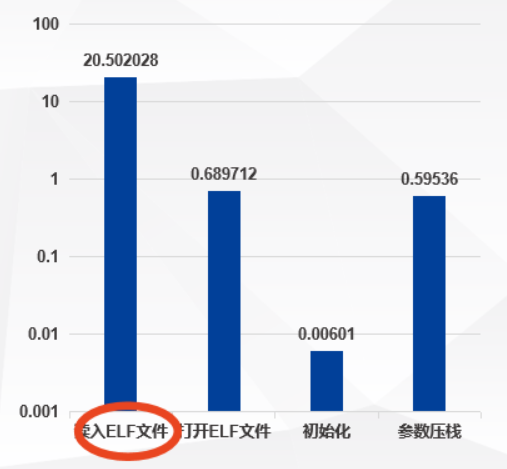
\includegraphics[scale=0.5]{figures/10-04/10-04-exec系统调用分析实验结果.png}
	\caption{exec系统调用分析实验结果}
	\label{exam-1}
\end{figure} 

笔者进行了Ultra OS的exec系统调用分析实验,主要方法是使用exec调用10次busybox,在系统内插入采集时延的观测点,利用日志输出相应时延数据。最后得到图\ref{exam-1}的结果。


不难发现,读入ELF文件的时延占整个系统调用时长的96.45\%,已然成为exec最长的关键路径。如果不能减少该部分的时间开销,将会很大程度上影响该系统调用的性能。

笔者进一步分析Ultra OS中exec系统调用加载elf文件的过程,得到如图\ref{exam-2}的结果。

\begin{figure}[htbp]
	\centering
	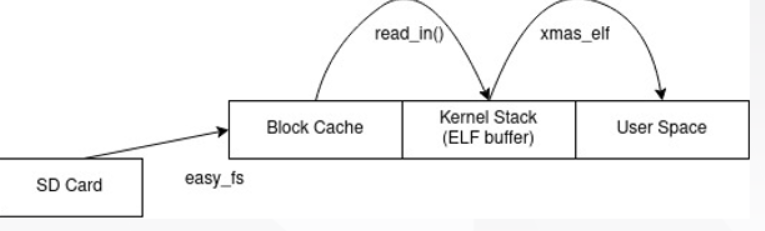
\includegraphics[scale=0.75]{figures/10-04/10-04-exec系统调用加载elf文件过程.png}
	\caption{exec系统调用加载elf文件过程}
	\label{exam-2}
\end{figure}

不难发现elf文件加载时延较大的原因是复制冗余,主要体现在:
\begin{itemize}
	\item \textbf{一次调用多次复制}。 elf文件内容需要从块缓存先拷贝到内核栈中的Elf buffer,再从Elf Buffer拷贝到用户空间,无形中增大了时延。
	
	\item \textbf{重复调用多次复制}。 每次读取同一elf文件时,没有缓存,需要重新完场图 中的过程,进一步增大时延。
\end{itemize}

为了解决该问题,NPUcore使用了写时复制、elf caching、零拷贝的方法,成功降低了复制冗余的问题。在与Ultra OS的对比实验中,NPUcore的时延均显著降低。

接下来详细介绍NPUcore对于exec系统调用的优化过程,读者可以通过图\ref{exam-3}辅助理解。

\begin{figure}[htbp]
	\centering
	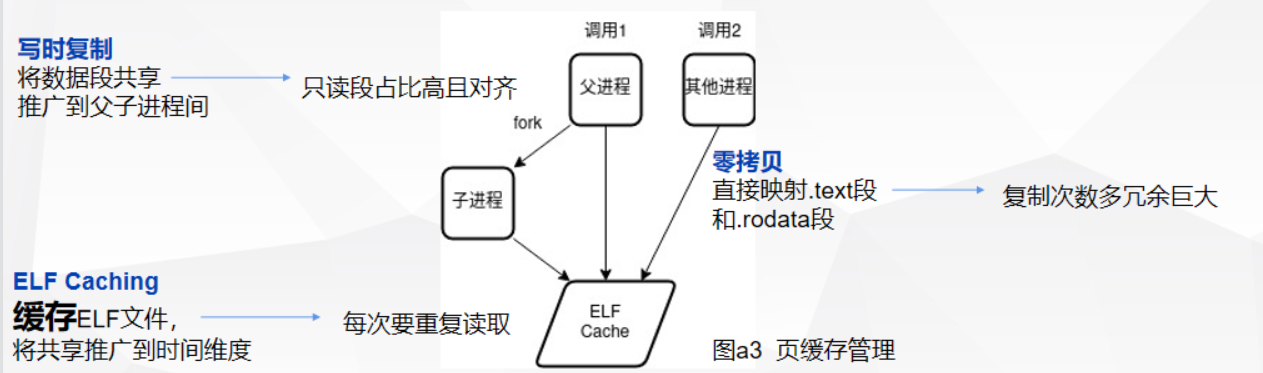
\includegraphics[scale=0.5]{figures/10-04/10-04-NPUcore对于exec系统调用的创新处理.png}
	\caption{NPUcore对于exec系统调用的创新处理}
	\label{exam-3}
\end{figure}

\textbf{优化目标}\;由于exec系统调用的主要延迟在于冗余拷贝,NPUcore的优化目标是减少拷贝,甚至做到多次变0次Copy或者只读文件。

\textbf{优化方法}\;利用RISC-V页表共享和缺页中断的特性,可以实现“需要时”直接使用ELF Cache内的ELF文件内容,而不需要再多次或重复Copy。需要时,指多次执行同一elf文件和父进程调用folk创建子进程时。

在以上优化思想的指导下,NPUcore添加了以下功能:

\textbf{写时复制}\;考虑到只读段内容占比高且对齐,NPUcore将数据段共享推广到父子进程间。

\textbf{elf caching}\;考虑到每次使用同一个elf文件时都要重复读取,NPUcore通过实现缓存ELF文件,将共享推广到时间维度。

\textbf{零拷贝}\;考虑到.text段和.rodata段映射过程中需要多次复制且冗余较大,NPUcore在.text段和.rodata段使用的是直接映射的方式。

\begin{figure}[htbp]
	\centering
	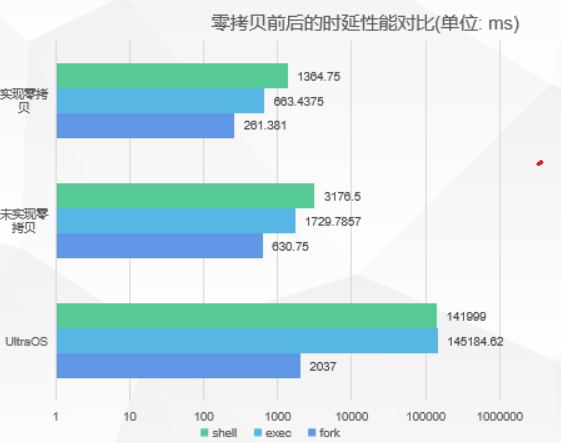
\includegraphics[scale=0.75]{figures/10-04/10-04-exec系统调用优化效果.png}
	\caption{exec系统调用优化效果}
	\label{exam-4}
\end{figure}

为了检验以上优化的效果,笔者设计实验比较时延性能对比。分别设置实现零拷贝,未实现零拷贝,Ultra OS三组,分别运行shell,exec,folk三个程序,记录时延,得到图\ref{exam-4}的结果。

可以看出零拷贝的性能比不实现零拷贝的性能高出1倍还多,而Ultra OS的性能由于冗余拷贝的存在,性能远不及前两组。

\subsection{时空优化2——文件系统缓存优化}

在文件系统章节,笔者介绍过PageCache和BufferCache,这些都是文件系统块缓存的部分,目的是为了缩小持久化设备和内存的读写速度差异。

\begin{figure}[htbp]
	\centering
	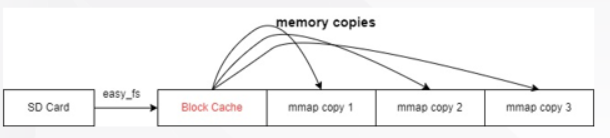
\includegraphics[scale=0.75]{figures/10-04/10-04-Ultra OS中的文件缓存过程.png}
	\caption{Ultra OS中的文件缓存过程}
	\label{exam-5}
\end{figure}

事实上,许多操作系统,包括清华大学的rCore以及哈工大的Ultra OS均实现了该功能。但是,以Ultral OS为例,其块缓存BlockCache设计中存在一个问题:在mmap系统调用时,多个进程调用同一个文件时,需要将文件内容分别拷贝到相应的进程空间,这就导致了多次数据拷贝的问题,造成了时延和空间上的冗余。图\ref{exam-5} 可以说明这一点。

NPUcore基于此进行优化,调整了块缓存的读写策略,从而省去了拷贝的过程,从而减少了时延和空间冗余,详细过程如下。

\textbf{优化目标} \; 减少不必要的拷贝(多次拷贝变一次拷贝)

\textbf{优化思想} \; 仍是利用RISC-V页表共享和缺页中断的特性,多个用户程序可以仅通过mmap系统调用建立的映射关系直接读写PageCache中的数据。

简而言之,就是用地址映射的方式,使得进程可以直接访问PageCache,从而省略了从PageCache拷贝数据的过程,图 解释了该过程。

\begin{figure}[htbp]
	\centering
	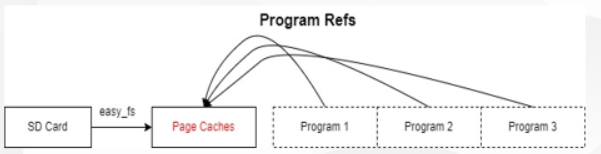
\includegraphics[height=8cm]{figures/10-04/10-04-NPUcore的文件缓存过程.png}
	\caption{NPUcore的文件缓存过程}
	\label{exam-6}
\end{figure}

\textbf{懒分配与写时复制}\; 图\ref{exam-7} 解释了两种写入情况,写时复制和直接写入。NPUcore使用了写入复制,当进程写入数据时复制PageCache,将数据写入复制后的PageCache。

\begin{figure}[htbp]
	\centering
	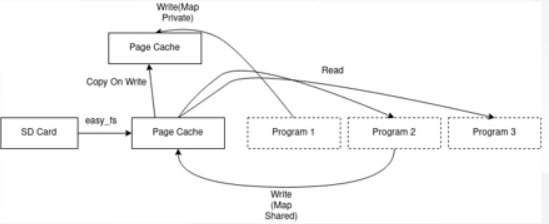
\includegraphics[scale=0.6]{figures/10-04/10-04-写时复制和直接写入.png}
	\caption{写时复制和直接写入}
	\label{exam-7}
\end{figure}

\textbf{页为单位} \; 块设备层的单位为块,而内存管理使用的单位为页。如果使用地址映射的方法访问cache则会出现单位问题,这也是为什么Ultra OS只能拷贝的原因。NPUcore这里设计了两个Cache,一个BufferCache用于缓存块设备中的数据,而PageCache实现块向页的转化。此过程可参考图\ref{exam-8}。

\begin{figure}[htbp]
	\centering
	\includegraphics[scale=0.6]{figures/10-04/10-04-NPUcore的PageCache.png}
	\caption{NPUcore的PageCache}
	\label{exam-8}
\end{figure}

\textbf{缓存与回收} \; 此部分与Cache相关。在文件系统中提到,整个内存地址空间均可以作为Cache的空间,所以只要空间足够就可以缓存数据,当内存已满时使用替换策略回收。

在实现了上述功能之后,笔者设计页缓存管理实验评估优化效果,分别使用旧缓存体系和新缓存体系分别测量mmap时延,分为file\_rd io\_read,file\_rd open\_to\_close和mmap_rd io\_rd.

\begin{figure}[htbp]
	\centering
	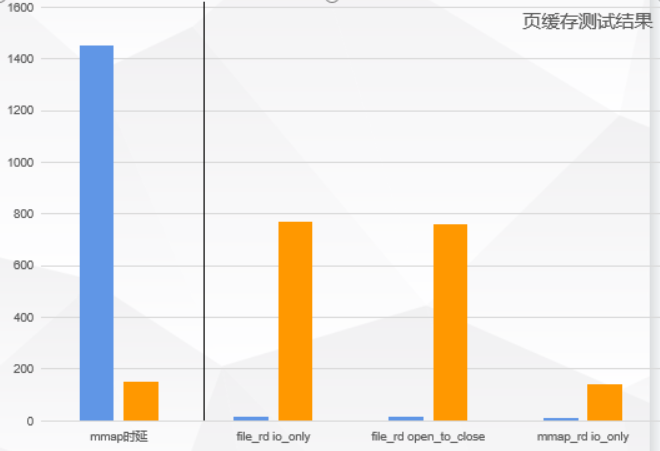
\includegraphics[scale=0.5]{figures/10-04/10-04-页缓存管理实验评估优化效果.png}
	\caption{页缓存管理实验评估优化效果}
	\label{exam-9}
\end{figure}

实验结果如图\ref{exam-9}所示。从图中可以看出,mmap的时延新缓存体系与旧缓存体系相比有了较大的降低,其他部分的数据却是旧缓存体系占优。由于多了一层cache,所以其他部分延迟的增加也是在意料之中。

\subsection{内存管理空间优化}

\textbf{问题提出与分析}

在多道程序运行时,存在内存空间不足的问题。具体而言如下:

1、如图\ref{fig:ELF}所示,测例本身的用户程序(ELF)占用的空间较大。

\begin{figure}[H]
	\centering
	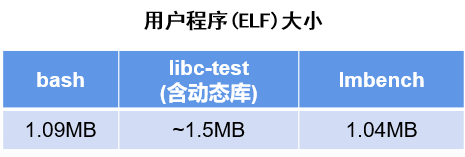
\includegraphics[width=0.6\textwidth]{figures/10-04-测例ELF.jpg}
	\caption{测例 ELF 大小}
	\label{fig:ELF}
\end{figure}

2、为了考验 os 对于内存管理的性能,部分测例在运行时,需要占用大量内存,比如在运行 libc-test 中的 sscanf_long 测例,需要申请 8M 的空间逐字节读写;在执行 lmbench 工具集中的 lat_ctx 测试时,需要进行 32,64,96 进程上下文切换的测试,不言而喻,这个过程需要占用大量的内存。

3、与此同时,还要受限于 k210 并不宽裕的内存大小,如图\ref{fig:k210}所示,k210 的内存空间已经捉襟见肘。

\begin{figure}[h]
	\centering
	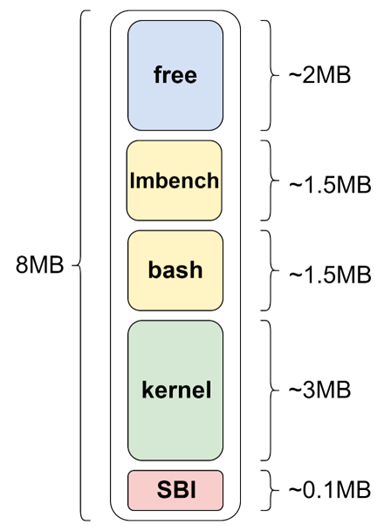
\includegraphics[width=0.38\textwidth]{figures/10-04-k210内存空间.jpg}
	\caption{k210 内存使用情况}
	\label{fig:k210}
\end{figure}

4、在前文所述的困难下,我们急需通过换出来腾空内存,从而实现内存的“扩容”。此时增加“换入换出”的功能似乎成为不二之选。但是在 NPUcore 之前, UltraOS 并没有实现这一功能(UltraOS 只有不完全的缺页处理和懒分配机制)。

5、如果采用换入换出的策略,又会遇到IO瓶颈, k210 上SD卡峰值读写速度约 1MB/s ,而 libc-test 每个测例限时 5s,如果不对内存管理进行优化,在运行测例时很容易就出现超时。

在以上种种限制之下,迫切需要一套集成优化方法来支持内存“扩容”。 


\textbf{优化方法与评估}

NPUcore内存采用了一套“扩容”集成优化方法,包括以下策略:

\begin{itemize}
	\item 懒分配(分配阶段)
	\item 缓存回收与写回 (回收)
	\item zRAM 压缩内存(压缩)
	\item 虚拟内存 换入换出(交换)
	\end{itemize}

具体而言,NPUcore 实现了一种依赖 Page Fault的优化(CoW)。通过将两个页表项的 W 权限位清零, 并且映射到相同的物理页。可以实现页面共享和写时复制(Copy on Write)。对共享页的写入会产生 Page Fault, 此时我们再结合内存描述符以及页表项的情况做出判断和相应处理。

如图\ref{fig:page fault}所示,是我们对相关 Fault 具体的处理方法:

\begin{figure}[h]
	\centering
	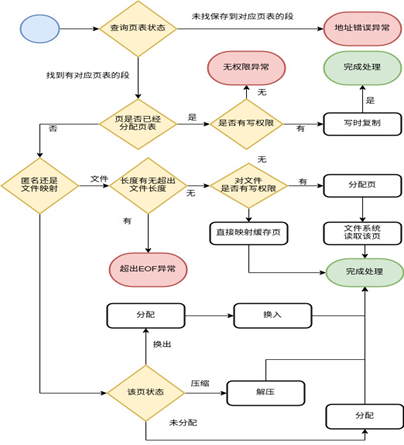
\includegraphics[width=0.65\textwidth]{figures/10-04-Page fault.jpg}
	\caption{Page Fault 处理方法}
	\label{fig:page fault}
\end{figure}

首先是 Segment fault,对于原本就没有权限的和没有映射的地址,会在页表状态(实际通过内存中的"MapArea"(段)结构储存)中查找失败, 然后直接进入无权异常/错地址异常(上方的两个红终止框)。

其次是 Page Fault 。由于没有权限的情况判断已经由之前的两个路径分支点完成, 这里一定是有权限的, 只是触发的权限是Read还是Write。进入这个分支的必然是页还没分配的,如果是文件映射,对于 MapArea 中有写入权限的, 按照Linux的默认行为, 是直接写回文件, 所以我们直接将页分配给这里, 然后读取一页的文件即可。对于文件没有写入权限的, 就可以直接映射已经缓存的页, 然后完成。之后的其他行为和别的已经映射的没有差异。事实上, Linux是允许阻断文件映射对源文件的写回, 但不是默认行为, 我们暂时不考虑。如果是匿名映射,则需要进行判断,如果该页面未被分配,则分配页面;如果是该页面已分配但是已被换出,则重新进行分配,即将该页面重新换入;如果该页面处于压缩内存当中,则将该页面进行解压,得到原来的页面,经过上述三种不同情况的处理,就可完成分配。

NPUcore 的“扩容”集成优化方法,效果极其显著。这一套虚拟内存管理方法,让应用程序可以感知到更多的可用内存,我们的实验也验证了 NPUcore 内存回收性能的高效。如图\ref{fig:memory test}所示,我们增加的内存管理方法,极大提升内存回收峰值,提高了操作系统的内存回收性能。

\begin{figure}[h]
	\centering
	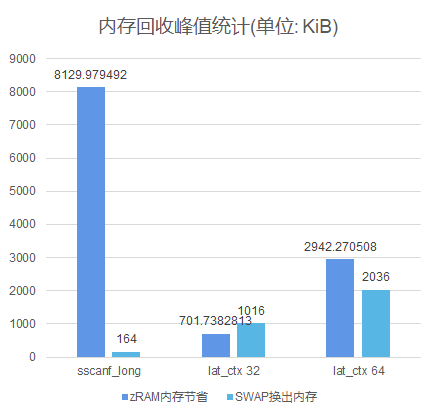
\includegraphics[width=0.56\textwidth]{figures/10-04-内存实验评估.jpg}
	\caption{NPUcore 内存回收性能比较}
	\label{fig:memory test}
\end{figure}


\subsection{可靠性优化:SD卡驱动优化}
、
\textbf{问题提出与分析}

在运行 libc-test 测试,k210 板 SD 卡驱动在运行多个用户程序时,内存占用率过高时会出现不稳定。 如图\ref{fig:SD error}所示,rCore Tutorial 系统在压力测试下SD卡驱动读写异常。

\begin{figure}[h]
	\centering
	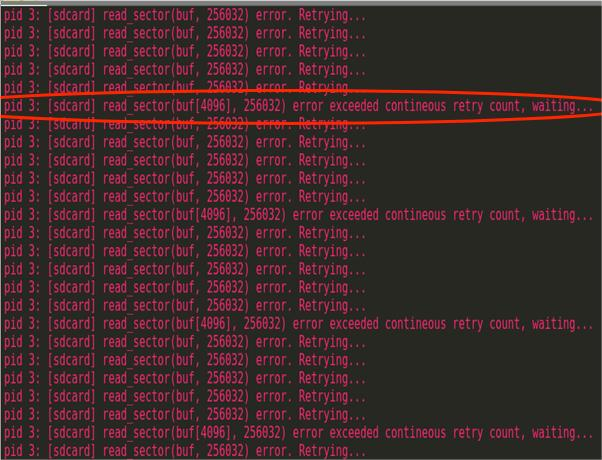
\includegraphics[width=0.55\textwidth]{figures/10-04-SD卡驱动异常.jpg}
	\caption{压力测试下SD卡驱动读写异常}
	\label{fig:SD error}
\end{figure}

我们经过初步分析,发现是因为测例在运行时访问了 KPU 内存,也就是高 2M 物理内存。进一步分析,我们发现问题出在当内存占用率高时,CPU 会频繁访问 KPU 内存,由于 KPU 与 CPU 的时钟频率不同,因此会造成访存不稳定,进而影响SD卡读写的稳定性。

\textbf{优化方法与评估}

为了让 NPUcore 在读写 SD 失败后具有错误恢复的能力 ,我们对 SD 卡驱动程序进行了完善,以提高 NPUcore 的稳定性。整个 SD 卡驱动恢复过程的伪代码如下所示。

\begin{algorithm}[tb]
	\caption{SD卡驱动恢复方法}
	\label{alg:sdcard recovery}
	\textbf{Input}: block\_id, buf\\
	\textbf{Output}: None~or~SUCCESS
	\begin{algorithmic}[1] %[1] enables line numbers
		
		\State \textbf{let} $result = self.write\_sector(buf, block\_id)$
		\State \textbf{let} $cont\_cnt = 0$
		
		\While{$result~~is~~error$ }
		\If{$cont\_cnt >= 0$}
		\State $log\_error("[sdcard]~~write\_sector(buf,~block\_id)~~error.~~Retrying...")$
		\State $result=self.write\_sector(buf,~block\_id)$
		\EndIf
		
		\State $cont\_cnt = cont\_cnt + 1$
		
		\If{$cont\_cnt >= 5$}
		\State $log\_error("[sdcard]~~write_sector(buf[length(buf)],~~block\_id)~~error~~exceeded~~continuous~~retry~~count,~~waiting...")$
		\State $self.wait\_for\_one\_second$
		
		\If{$self.write\_sector(buf,~block\_id)$ is error}
		\State $self.init$
		\State $self.wait\_for\_one\_second$
		\Else
		\State \textbf{break}
		\EndIf
		
		\State $cont\_cnt = 0$
		\EndIf
		\EndWhile
	\end{algorithmic}
\end{algorithm}

正如伪代码所示,在具体的实现上,NPUcore 的 SD 卡驱动恢复方法为:

首先会进行错误判断,如果SD卡驱动读写没完成则会导致失败(SD卡驱动崩溃后驱动函数会返回错误信息)。

至于失败后的恢复过程,多数情况下,会进行5次尝试读写,如果全部失败(返回错误信息), 则等待1秒,再1次尝试读写;如果再失败,则直接重新初始化整个驱动,再重复整个恢复过程,直到成功。

NPUcore 的 SD 卡驱动恢复方法,成效显著。为了验证其效果,使用下列命令:

\begin{lstlisting}[language=bash]
	while true; do 
	   ./run-all.sh; 
	done
\end{lstlisting}

进行压力测试,如图\ref{fig:SD recovery}所示。最终,NPUcore 可以在 k210 开发板上连续正确运行6个小时!这项改进也被其他参赛队伍引用

\begin{figure}[h]
	\centering
	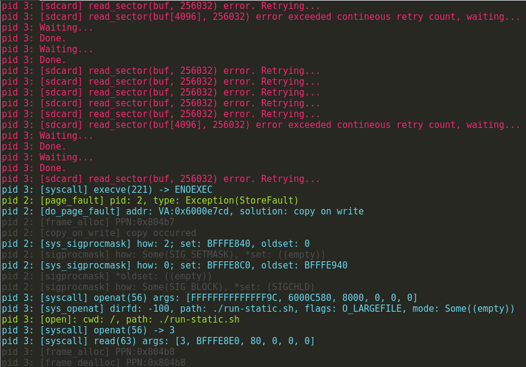
\includegraphics[width=0.55\textwidth]{figures/10-04-SD卡驱动读写错误恢复方法效果实验评估.png}
	\caption{SD卡驱动恢复方法效果实验评估}
	\label{fig:SD recovery}
\end{figure}


